% TEMPLATE.TEX
%
% Time-stamp: <2013-03-26 11:09 olenz>
%
% This is an extensively documented LaTeX file that shows how to
% produce a good-looking document with current LaTeX (11/2012).
%
% IMPORTANT!
%
%   Some obsolete commands and packages
% ----------|-------------------------------
% obsolete  |     Replacement in LATEX 2ε
% ----------|-------------------------------
%           | local            global/switch
% ----------|-------------------------------
% {\bf ...} | \textbf{...}     \bfseries
%     -     | \emph{...}       \em
% {\it ...} | \textit{...}     \itshape
%     -     | \textmd{...}     \mdseries
% {\rm ...} | \textrm{...}     \rmfamily
% {\sc ...} | \textsc{...}     \scshape
% {\sf ...} | \textsf{...}     \sffamily
% {\sl ...} | \textsl{...}     \slshape
% {\tt ...} | \texttt{...}     \ttfamily
%     -     | \textup{...}     \upshape
%
% DON'T USE \\ TO MAKE LINEBREAKS, INSTEAD JUST LEAVE A BLANK LINE!
%
\RequirePackage[l2tabu,orthodox]{nag} % turn on warnings because of bad style
\documentclass[a4paper,10pt,bibtotoc]{scrartcl}
%
\usepackage[bottom=3.5cm, top=3cm]{geometry}
\usepackage{subcaption}
\captionsetup[subfigure]{list=true, position=top}
\usepackage{float}
%%%%%%%%%%%%%%%%%%%%%%%%%%%%%%%%%%%%
% KOMA CLASSES
%%%%%%%%%%%%%%%%%%%%%%%%%%%%%%%%%%%%
%
% The class "scrartcl" is one of the so-called KOMA-classes, a set of
% very well done LaTeX-classes that produce a very European layout
% (e.g. titles with a sans-serif font).
%
% The KOMA classes have extensive documentation that you can access
% via the commands:
%   texdoc scrguide # in German
%   texdoc scrguien # in English
%
%
% The available classes are:
%
% scrartcl - for "articles", typically for up to ~20 pages, the
%            highest level sectioning command is \section
%
% scrreprt - for "reports", typically for up to ~200 pages, the
%            highest level sectioning command is \chapter
%
% scrbook  - for "books", for more than 200 pages, the highest level
%            sectioning command is \part.
%
% USEFUL OPTIONS
%
% a4paper  - Use a4 paper instead of the default american letter
%            format.
%
% 11pt, 12pt, 10pt
%          - Use a font with the given size.
%
% bibtotoc - Add the bibliography to the table of contents
%
% The KOMA-script classes have plenty of options to modify

% This allows to type UTF-8 characters like ä,ö,ü,ß
\usepackage[utf8]{inputenc}

\usepackage[T1]{fontenc}        % Tries to use Postscript Type 1 Fonts for better rendering
\usepackage{lmodern}            % Provides the Latin Modern Font which offers more glyphs than the default Computer Modern
\usepackage[intlimits]{amsmath} % Provides all mathematical commands
\usepackage{amssymb}
\usepackage{hyperref}           % Provides clickable links in the PDF-document for \ref
\usepackage{graphicx}            % Allow you to include images (like graphicx). Usage: \includegraphics{path/to/file}

% Allows to set units
\usepackage[ugly]{units}        % Allows you to type units with correct spacing and font style. Usage: $\unit[100]{m}$ or $\unitfrac[100]{m}{s}$

% Additional packages
\usepackage{url}                % Lets you typeset urls. Usage: \url{http://...}
\usepackage{breakurl}           % Enables linebreaks for urls
\usepackage{xspace}             % Use \xpsace in macros to automatically insert space based on context. Usage: \newcommand{\es}{ESPResSo\xspace}
\usepackage{xcolor}             % Obviously colors. Usage: \color{red} Red text
\usepackage{booktabs}           % Nice rules for tables. Usage \begin{tabular}\toprule ... \midrule ... \bottomrule
\usepackage{siunitx}


% Source code listings
\usepackage{listings}           % Source Code Listings. Usage: \begin{lstlisting}...\end{lstlisting}
\lstloadlanguages{python}
\definecolor{lightpurple}{rgb}{0.8,0.8,1}

\lstset{
stepnumber=1,
numbersep=5pt,
numberstyle=\small\color{black},
basicstyle=\ttfamily,
%keywordstyle=\color{black},
%commentstyle=\color{black},
%stringstyle=\color{black},
frame=single,
tabsize=4,
language = python,
backgroundcolor=\color{black!5}}

\usepackage{float}

\begin{document}

\titlehead{Simulation Methods in Physics I \hfill WS 2019/2010}
\title{Report for Worksheet 5: Monte Carlo}
\author{Markus Baur and David Beyer}
\date{\today}
\maketitle

\tableofcontents
\section{Simple Sampling -- Integration}
The Python code for the following section can be found in the file ex\_5\_2.py.
\subsection{Exact Integration}
A plot of the function $f(x)$ on the interval $\left[0.1,50.0\right]$ is shown in \autoref{fig:fig1}. 
We can see that the function is almost zero for most values of $x$, disrupted by sharp peaks.
This means that we will need a lot of samples to obtain an acceptable value using simple sampling.
\begin{figure}
	\centering
	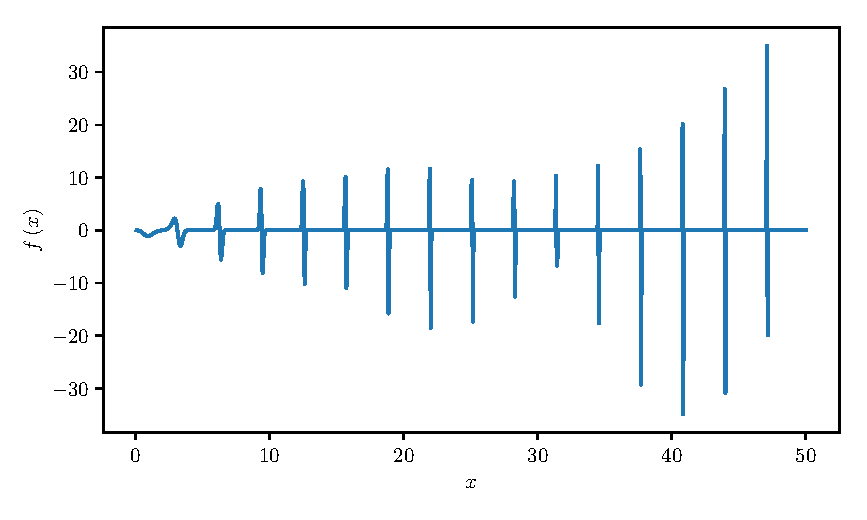
\includegraphics[width=\linewidth]{plotf.pdf}
	\caption{Plot of the function $f(x)$ on the interval $\left[0.1,50.0\right]$.}
	\label{fig:fig1}
\end{figure}

To obtain the exact integral of $f(x)$ over an interval $\left[a, b\right]$, we wrote the function exact\_integral, which uses the SymPy module to calculate a closed expression of the integral:
\begin{lstlisting}
def exact_integral(a, b):
    x = Symbol('x')
    ret = integrate((-2 * x**2 * sin(x) * cos(x) - 2 * x * sin(x)**2)\
        * exp(-x**2 * sin(x)**2), (x, a, b))
    return ret
\end{lstlisting}
The obtained value is
\begin{align}
\int_{0.1}^{50.0}\mathrm{d}x\,f(x)\approx -0.9999.
\end{align}


\subsection{Monte Carlo Integration}
To perform a Monte Carlo integration using simple sampling, we wrote the following function:
\begin{lstlisting}
def simple_sampling(f, a, b, N):
    dx = (b - a) / N
    ret = 0.0
    sample = 0.0
    squared_sum  = 0.0
    for i in range(N):
        sample = f((b - a) * np.random.random_sample() + a)
        ret += sample
        squared_sum += sample ** 2
    error = np.sqrt(squared_sum - (ret ** 2) / N)
    error *= (b - a) / np.sqrt(N * (N-1))
    ret *= dx
    return ret, error
\end{lstlisting}
The has as its arguments the function $f$ which has to be integrated, the limits $a$ and $b$ of the interval and the number of samples $N$. 
Furthermore, the function also calculates the an estimate for the error of the calculated value.

To compute an estimate of the error for the obtained integral, we note that the $N$ different samples $f(x_i)$ are uncorrelated in the case of simple sampling.
The unbiased estimator of the variance of $f$ is given by
\begin{align}
\hat{\sigma}(f)^2 = \frac{1}{N-1}\left(\sum_{i=1}^{N}f(x_i)^2-\frac{1}{N}\left(\sum_{i=1}^{N}f(x_i)\right)^2\right).
\end{align}
Because the samples are uncorrelated and statistically independent, we can calculate the unbiased estimator of the variance of the integral $I$ as
\begin{align}
\hat{\sigma}(I)^2 &= \frac{\left(a-b\right)^2}{N^2}\sum_{i=1}^{N} \hat{\sigma}(f)^2 = \frac{\left(a-b\right)^2\hat{\sigma}(f)^2}{N}\\
&=\frac{\left(a-b\right)^2}{N\left(N-1\right)}\left(\sum_{i=1}^{N}f(x_i)^2-\frac{1}{N}\left(\sum_{i=1}^{N}f(x_i)\right)^2\right)
\end{align}
which leads to an estimation of the error of $I$ that is given by
\begin{align}
\epsilon(I)=\sqrt{\frac{\left(a-b\right)^2}{N\left(N-1\right)}\left(\sum_{i=1}^{N}f(x_i)^2-\frac{1}{N}\left(\sum_{i=1}^{N}f(x_i)\right)^2\right)}.
\end{align}
This error estimation is equal to the estimator for the standard error of the mean of $f$ times the length of the interval $[a,b]$, which is not surprising considering that $I$ is given by $\left(b-a\right)\cdot \overline{f}$.




\section{Importance Sampling -- Metropolis-Hastings Algorithm}
\section{Simulate the Ising Model}
\subsection{Exact Summation}
\subsection{Monte Carlo Simulation}
\subsection{Error Analysis}

\end{document}
